\documentclass{article}
\usepackage[utf8]{inputenc}
\usepackage{graphicx,amsmath,amsfonts,amssymb}

\title{SVVR Assignment 1}
\author{Sander Nugteren (6042023) \and Merel de Groot ()}
\date{November 2014}

\begin{document}

\section{Data types}
For this assignment a dataset of cars has to be visualised. The data consists
of the following variables:\\\\
\begin{tabular}{|l|l|}
	\hline
	Variable & Data type \\
	\hline
	Model & nominal \\
	Miles per Gallon & quantity \\
	Cylinders & quantity \\
	Horsepower & quantity \\
	Weight & quantity \\
	Year & quantity \\
	Origin & nominal\\
	\hline
\end{tabular}

\section{Visual Attribute Choice}
The most important things to show in the visualization in our opinion are the
quantity data types. Because the value ranges for miles per gallon, horsepower and
weight are the largest of the quantitative data, we opted to
use the x, y and z axes for these variables. For the cylinders we use shapes,
and for the year we use color intensity. The origin, as it is a nominal
variable, is represented by color. Since model is a nominal datatype with a
huge range, it is difficult to represent. We tried to label the datapoints with
the model names at first, but this cluttered up the data too much.

\section{The visualization}

\begin{figure}
	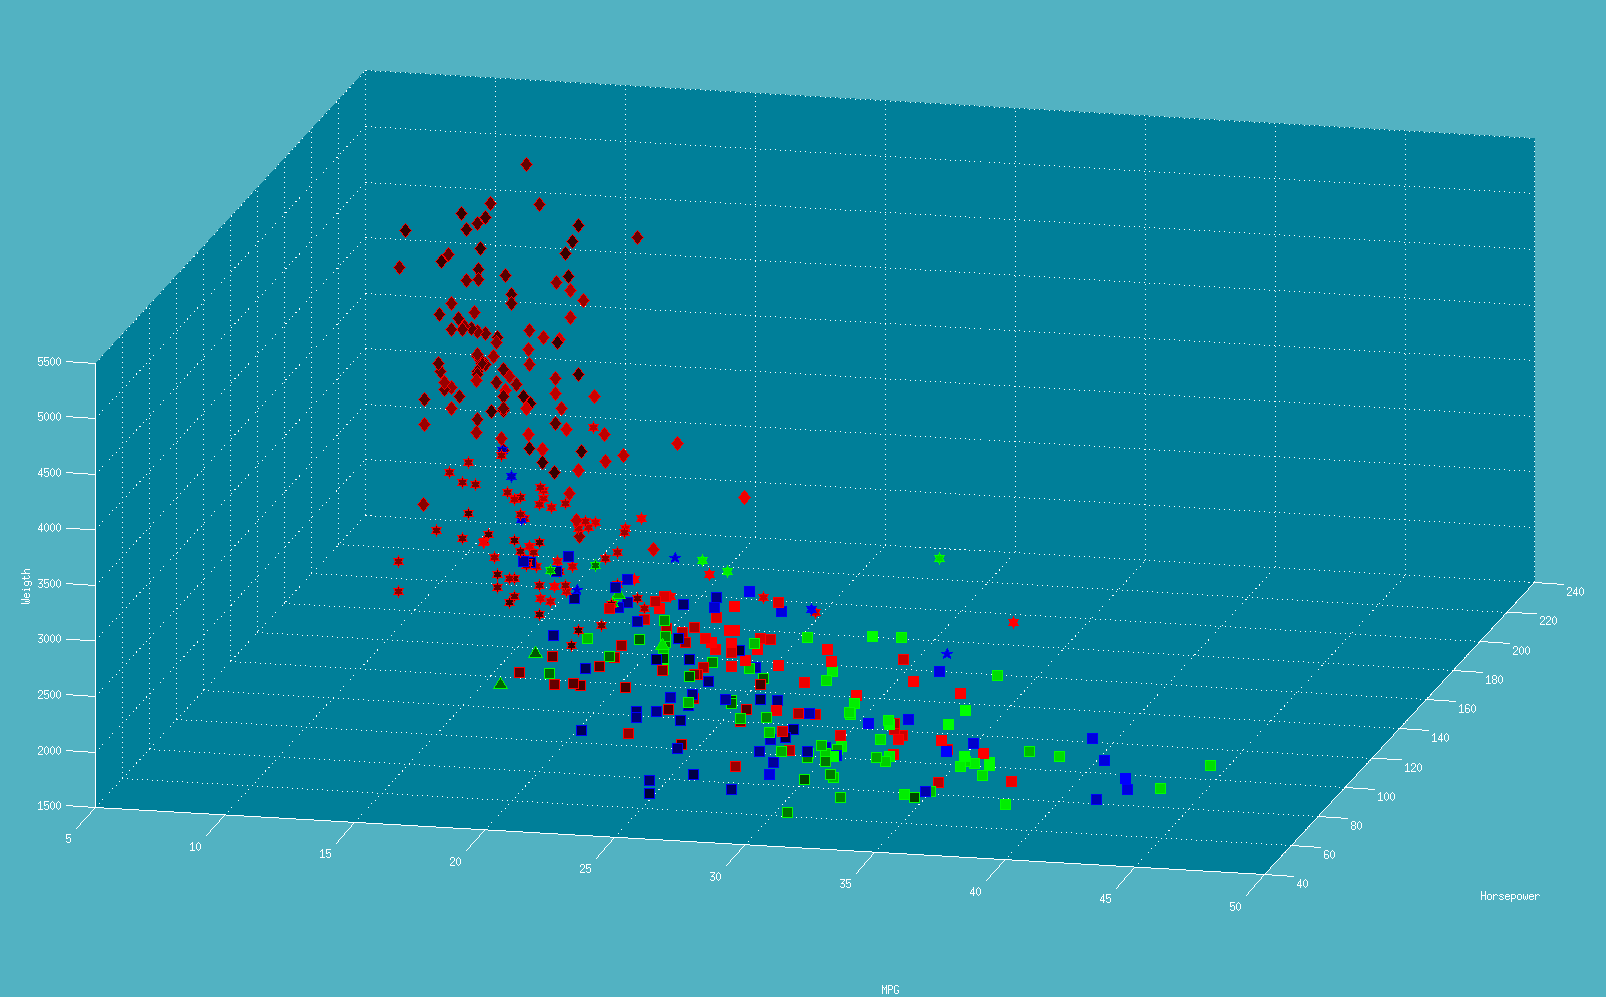
\includegraphics{scivis_plot}
	\caption{American cars are displayed in red, Japanes ones in green and
	European ones in blue.}
\end{figure}

We can see many things in this graph. For example, American cars tend to have
lots of cylinders, are heavier and less efficient but have lots of horsepower,
while Japanese cars are lighter and more efficient, but have less horsepower.
Also, the correlation between horsepower and cylinder amount is clearly
visible.

\end{document}
